\appendix
\addcontentsline{toc}{chapter}{Appendici}
\chapter[Riepilogo complessità computazionale]{Riepilogo sulla teoria di complessità 
computazionale}
\label{chap:appA}
In questa appendice verranno riepilogati i concetti base della teoria di complessità 
computazionale.

La Sezione \ref{sec:complessitaAlgoritmi} descrive in termini generali la 
complessità di un generico algoritmo in base alla dimensione dell'istanza.

La Sezione \ref{sec:complessitaProblemi} descrive invece le varie classi di complessità 
in cui si possono suddividere i problemi.

\section{Complessità degli algoritmi}
\label{sec:complessitaAlgoritmi}
La teoria della complessità algoritmica ha come obiettivo la stima di quanto onere 
computazionale è richiesto a un algoritmo per risolvere un dato problema $P$, per poter 
selezionare l'algoritmo più efficiente. Le metriche per la misura della complessità 
computazionale di un algoritmo sono:
\begin{itemize}
 \item Complessità spaziale: occupazione di memoria richiesta;
 \item Complessità temporale: tempo di calcolo.
\end{itemize}
La misura è effettuata stimando il numero di operazioni elementari necessarie per 
risolvere un'\emph{istanza} $I$ del problema $P$. Chiaramente, il tempo e lo spazio 
impiegati dipendono soprattutto dalla dimensione dell'istanza $\vert I \vert$, per questo 
la stima della complessità sarà una funzione di $n$ (che cambia a seconda della 
dimensione dell'istanza).

Per il calcolo si considera la rapidità di crescita del numero di operazioni elementari 
effettuate dall'algoritmo nel caso peggiore.
\begin{mydef}
\label{def:definizioneComplessita}
Dato il numero di operazioni per 
risolvere un'istanza $I$ di un problema $P$,
\begin{displaymath}
 I \leq f(n), \quad \forall I\  \text{con}\  \vert I \vert \leq n
\end{displaymath}
si dice che $f(n)$ è dell'ordine di $g(n)$ e si scrive $f(n) = O(g(n))$ se
\begin{equation}
 \exists c > 0\  \vert\  f(n) \leq c\cdot g(n)
\end{equation}
per $n$ sufficientemente grande.
\end{mydef}

Seguendo la Definizione \ref{def:definizioneComplessita}, un algoritmo è detto 
\emph{polinomiale} se necessita di un numero di operazioni elementari
\begin{displaymath}
 f(n) = O(n^d) \quad \text{con}\  n = \vert I \vert, d\  \text{costante}
\end{displaymath}
Similmente, un algoritmo è detto \emph{esponenziale} se necessita di un numero di 
operazioni elementari
\begin{displaymath}
 f(n) = O(2^n) \quad \text{con}\ n = \vert I \vert
\end{displaymath}

Ad esempio il merge-sort, un algoritmo per l'ordinamento di un array di $n$ interi, ha 
complessità computazionale dell'ordine di $O(n\cdot \log n)$.

Nella prossima sezione verrà trattata la complessità intrinseca dei problemi che possono 
essere risolti algoritmicamente.

\section{Complessità dei problemi}
\label{sec:complessitaProblemi}
Mentre lo studio della complessità degli algoritmi consente di classificare alcuni 
algoritmi come migliori rispetto ad altri nel risolvere un determinato problema, lo 
studio della complessità dei problemi consente di stimarne la difficoltà intrinseca, 
ovvero quanto può essere efficiente il miglior algoritmo che può risolvere un problema.

\begin{mydef}
 Un problema di ottimizzazione $P$ è detto \emph{polinomiale} se ogni sua istanza è 
risolvibile da un algoritmo di complessità polinomiale.
\end{mydef}
I problemi risolvibili in tempo polinomiale sono generalmente ritenuti ``facili''. Nella 
teoria della $\mathcal{NP}$-completezza si classificano, oltre a questi, anche altri 
problemi per i quali non esiste un algoritmo che li risolva in tempo polinomiale.

Nella teoria della complessità ci si focalizza sui \emph{problemi di decisione}, anche 
definiti \emph{problemi di riconoscimento}:
\begin{mydef}
 Un problema di decisione è un problema che ammette solo una risposta: ``si''/``no''.
\end{mydef}

Dato un problema di ottimizzazione, è sempre possibile associare ad esso un problema di 
decisione. Ad esempio, il problema del commesso viaggiatore\footnote{In inglese \ac{TSP}, 
è formulato come segue: dato un grafo $G = (N, A)$ orientato, con costi associati agli 
archi, determinare un circuito di costo minimo che consenta di visitare esattamente una 
volta ogni nodo.} è riconducibile al seguente problema di decisione:
\begin{quotation}
Dato un grafo $G = (N, A)$ con costi $c_{ij} \; \forall (i,j) \in A$ e 
un intero $L$, esiste un circuito hamiltoniano\footnote{Un circuito è detto 
\emph{hamiltoniano} se passa esattamente una volta per ogni nodo.} $C$ tale che
\begin{displaymath}
 \sum_{(i,j) \in C}c_{ij} \leq L\text{?}
\end{displaymath}
\end{quotation}
La complessità intrinseca di un problema di ottimizzazione si stima dunque partendo dal 
corrispondente problema di decisione, se tale problema è difficile il problema di 
ottimizzazione è almeno altrettanto difficile.

Verranno ora enumerate le varie classi di complessità dei problemi di decisione.

\paragraph{Classe di complessità $\mathcal{P}$}
\begin{mydef}
La classe di complessità $\mathcal{P}$ comprende i problemi di decisione che possono 
essere risolti in tempo polinomiale.
\end{mydef}
Per ogni problema di ottimizzazione appartenente a questa classe esiste quindi un 
algoritmo che per ogni istanza del problema risponde ``si''/``no'' in tempo polinomiale 
rispetto alla dimensione dell'istanza.

Esempi di problemi di questo tipo sono relativi ai problemi di cammini minimi, nella 
ricerca operativa.

\paragraph{Classe di complessità $\mathcal{NP}$}
\begin{mydef}
 La classe di complessità $\mathcal{NP}$ comprende i problemi di decisione 
tali che le istanze con risposta affermativa possono essere verificate in tempo 
polinomiale.
\end{mydef}
$\mathcal{NP}$ non significa ``Non Polinomiale'', bensì ``Non-deterministico 
Polinomiale''.

\begin{figure}[ht]
 \begin{center}
  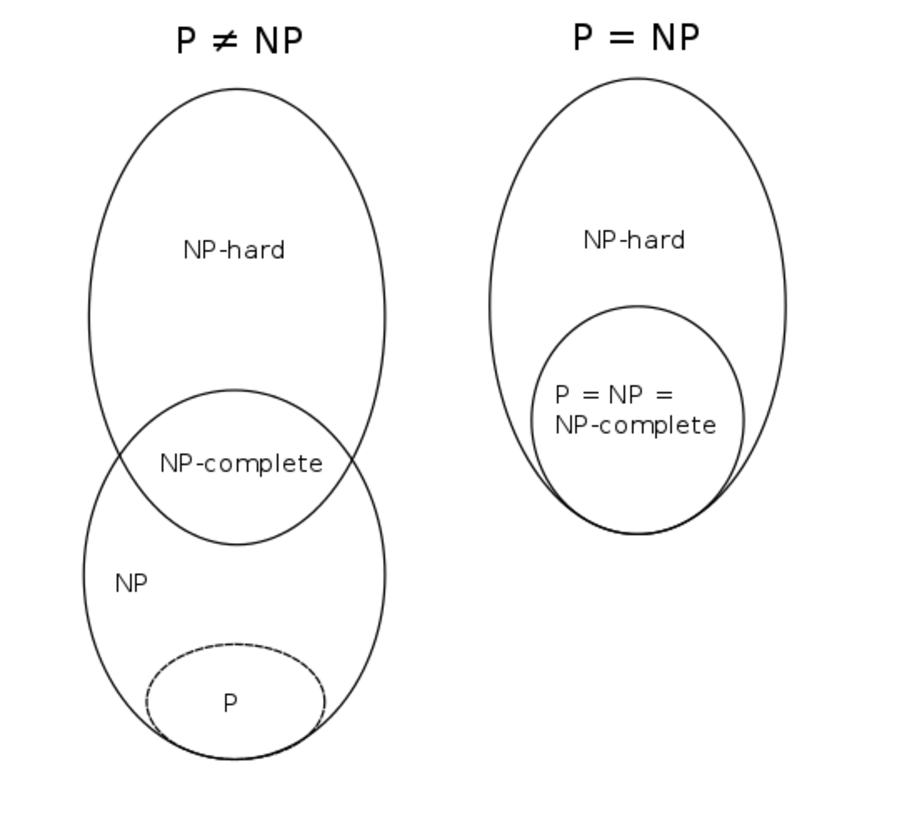
\includegraphics[width=0.7\textwidth]{appendici/figure/ClassiComplessita.pdf}
  \caption{Classi di complessità dei problemi.}
  \label{fig:ClassiComplessita}
 \end{center}
\end{figure}


Vale la relazione $\mathcal{P} \subseteq \mathcal{NP}$, ma la questione attualmente più 
importante nella teoria della complessità è se questa inclusione sia stretta oppure 
no, ovvero se $\mathcal{P} \subset \mathcal{NP}$ ed esista un problema di classe 
$\mathcal{NP}$ che non sia compreso in $\mathcal{P}$ \cite{GasarchPoll} (vedi Figura 
\ref{fig:ClassiComplessita}).

Nel prossimo paragrafo verrà trattato il concetto di \emph{riduzione polinomiale} fra 
problemi, fondamentale per capire le ultime due classi di problemi: i problemi 
$\mathcal{NP}$-completi e i problemi $\mathcal{NP}$-difficili.

\subparagraph{Riduzione polinomiale fra problemi}
Il concetto di riduzione polinomiale\footnote{Detta anche \emph{Turing-riduzione in tempo 
polinomiale}.} consente di ordinare i problemi di decisione, definendo quelli più 
difficili.

\begin{mydef}
 Dati due problemi $P_1, P_2 \in \mathcal{NP}$, $P_1$ si riduce in tempo polinomiale a 
$P_2$ e si scrive $P_1 \propto P_2$, se esiste un algoritmo per la risoluzione di $P_1$ 
che:
\begin{itemize}
 \item Chiama un dato numero di volte un algoritmo per la risoluzione di $P_2$,
 \item Risulta polinomiale, nell'ipotesi che l'algoritmo per la risoluzione di $P_2$ 
richieda una sola unità di tempo.
\end{itemize}
\end{mydef}
Come conseguenza, se $P_1 \propto P_2$ e $P_2$ può essere risolto utilizzando un 
algoritmo di complessità polinomiale, anche $P_1$ può essere risolto in tempo polinomiale.

Questa definizione consente di illustrare le rimanenti classi di problemi.

\paragraph{I problemi $\mathcal{NP}$-completi}
\begin{mydef}
 Un problema $P$ è $\mathcal{NP}$-completo se e solo se:
 \begin{enumerate}
  \item $P \in \mathcal{NP}$,
  \item $\forall P' \in \mathcal{NP} \setminus \left\{P\right\}, \quad P' \propto P$.
 \end{enumerate}
\end{mydef}
La $\mathcal{NP}$-completezza è quindi un forte indizio di difficoltà intrinseca di un 
problema; infatti, se un problema $\mathcal{NP}$-completo fosse risolvibile in tempo 
polinomiale, lo sarebbe infatti qualsiasi problema in $\mathcal{NP}$\footnote{Infatti, in 
questo caso si avrebbe che $\mathcal{P} = \mathcal{NP}$, eventualità non ancora 
dimostrata ma considerata improbabile.}.

Il primo problema ad essere dimostrato $\mathcal{NP}$-completo è il problema della 
soddisfacibilità booleana (SAT)\footnote{Consiste nel determinare se una formula booleana 
sia soddisfacibile oppure no, ovvero determinare se esiste un assegnamento di valori alle 
variabili che rende vere tutte le clausole della formula.}, dimostrazione fornita da 
Stephen Cook in \cite{CookSAT}, che in tale pubblicazione formalizza inoltre la nozione 
di riduzione polinomiale vista nel precedente paragrafo.

\paragraph{I problemi $\mathcal{NP}$-difficili}
\begin{mydef}
 Un problema $P_1$ è $\mathcal{NP}$-difficile se e solo se esiste un problema $P_2$ 
$\mathcal{NP}$-completo riducibile in tempo polinomiale a $P_1$, cioè 
$P_2 \propto P_1$.
\end{mydef}
In maniera informale, i problemi $\mathcal{NP}$-difficili possono essere definiti come 
``almeno altrettanto difficili rispetto ai più difficili problemi in $\mathcal{NP}$'' (i 
problemi $\mathcal{NP}$-completi). Mentre la classe di complessità $\mathcal{NP}$ 
comprende problemi di decisione, i problemi $\mathcal{NP}$-difficili possono essere 
di qualsiasi tipo: problemi di decisione, di ottimizzazione o di ricerca. Questo 
implica che tutti i problemi di ottimizzazione la cui versione di decisione è 
\mbox{$\mathcal{NP}$-completa} sono $\mathcal{NP}$-difficili.
